\chapter{Khảo sát nhu cầu, hiện trạng và định hướng thiết kế}
\label{Chapter2}

Chương 1 đặt vấn đề sử dụng AI trong xét duyệt bài báo dưới các ràng buộc về liêm chính, quyền hạn và trách nhiệm học thuật. Chương 2 xem xét vấn đề này dựa trên ba nguồn: nhu cầu người dùng, quy trình nghiệp vụ của các nền tảng hiện có và xu hướng phát triển nền tảng lấy AI làm trọng tâm, tức xem AI là một năng lực cốt lõi của sản phẩm. Mục tiêu của chương không phải chứng minh ConferenceSpace ưu việt hơn các hệ thống được khảo sát, mà xác định tác vụ nào phải dựa trên quy trình nghiệp vụ ổn định, tác vụ nào cần được xử lý bằng thuật toán cố định, có thể kiểm chứng và tác vụ nào phù hợp với luồng AI hỗ trợ có kiểm soát.

Mạch lập luận của chương gồm bốn bước. Mục 2.1 trình bày khảo sát nhu cầu theo ba vai trò Tác giả, Phản biện viên và Chủ tọa. Mục 2.2 đối chiếu hai nhóm nền tảng: nhóm đã hoàn thiện quy trình nghiệp vụ, được dùng để xác lập chuẩn tham chiếu cho vòng đời xét duyệt, và nhóm lấy AI làm trọng tâm, được dùng để nhận diện các khâu tích hợp AI cùng ranh giới trách nhiệm đã công bố. Mục 2.3 chuyển kết quả khảo sát thành các vấn đề thiết kế theo mức độ nghiêm trọng của hậu quả do từng tác vụ có thể gây ra. Cuối cùng, Mục 2.4 đặc tả yêu cầu và quy ước trách nhiệm, sau đó chỉ ra bằng chứng tương ứng ở Chương 4. Mô hình ba lớp là một lựa chọn thiết kế của đề tài, không phải kiến trúc tối ưu đã được các tài liệu khảo sát chứng minh.

\section{Khảo sát nhu cầu người dùng}

\subsection{Mục tiêu khảo sát}

Nhóm thực hiện khảo sát nhu cầu để xác định những khó khăn thực tế của người dùng khi tham gia quy trình hội nghị khoa học, đặc biệt trong các hoạt động nộp bài, theo dõi trạng thái, phản biện và điều phối hội nghị. Khảo sát không đại diện cho toàn bộ cộng đồng học thuật mà cung cấp dữ liệu định hướng để nhận diện những vấn đề có thể ảnh hưởng trực tiếp đến thiết kế sản phẩm.

Khảo sát tập trung vào ba câu hỏi:

\begin{itemize}
    \item Người dùng đang gặp khó khăn gì khi sử dụng các nền tảng như EasyChair, Microsoft CMT hoặc OpenReview?
    \item Những chức năng nào được người dùng kỳ vọng nhất trong một nền tảng quản lý hội nghị mới?
    \item Người dùng chấp nhận AI ở mức nào, và họ muốn giữ quyền kiểm soát ra sao khi AI tham gia vào quy trình học thuật?
\end{itemize}

Cách đặt câu hỏi này bám sát ranh giới đã nêu ở Chương 1: AI có thể hỗ trợ nhập liệu, kiểm tra, đọc hiểu và tổng hợp thông tin, nhưng không được thay thế quyết định học thuật của con người.

\subsection{Đối tượng và đặc điểm mẫu khảo sát}

Khảo sát thu được 71 phản hồi từ những người đang học tập, nghiên cứu hoặc làm việc trong môi trường có liên quan đến hội nghị khoa học. Các nhóm chính gồm sinh viên đại học và học viên cao học, giảng viên và nhà nghiên cứu, cùng người làm việc tại doanh nghiệp có tham gia hoạt động nghiên cứu.

\begin{figure}[htbp]
    \centering
    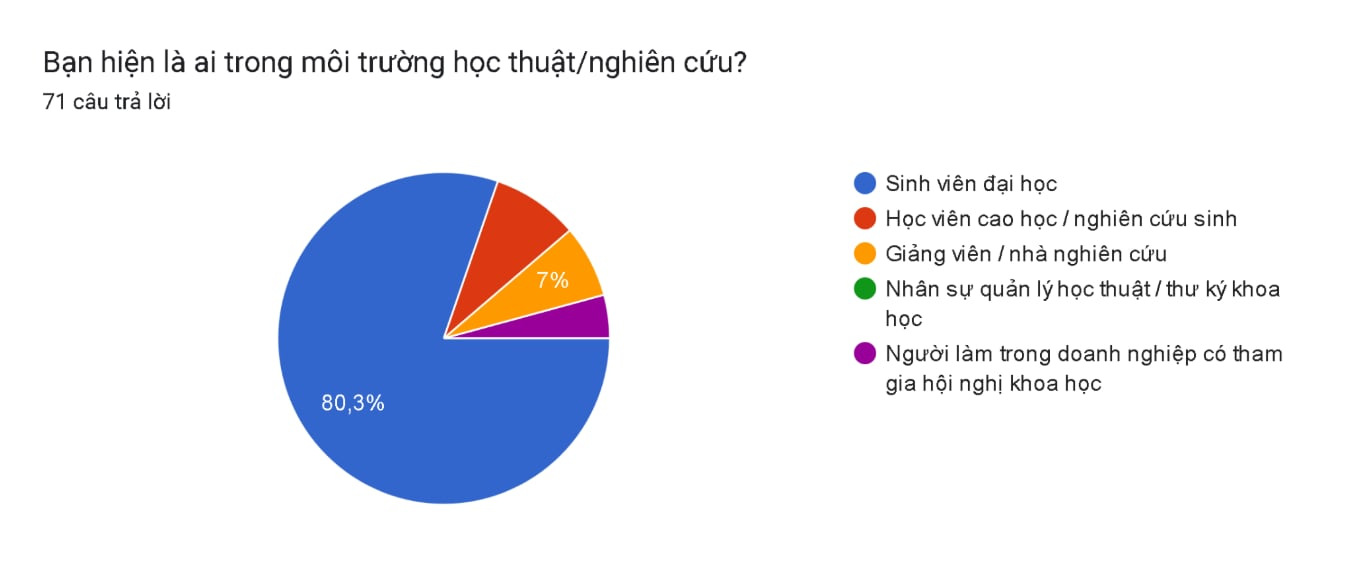
\includegraphics[width=0.9\textwidth]{images/chapter_2_picture_1.jpg}
    \caption{Phân bố đối tượng tham gia khảo sát}
    \label{fig:ch2-survey-participants}
\end{figure}

Hình~\ref{fig:ch2-survey-participants} trình bày phân bố mẫu khảo sát theo vai trò hoặc nhóm nghề nghiệp. Thành phần mẫu là cơ sở để xác định phạm vi diễn giải kết quả.

Trong phạm vi đề tài, ba nhóm vai trò được quan tâm nhất là:

\begin{itemize}
    \item \textbf{Tác giả:} người nộp bài, cần quy trình nộp bài dễ hiểu, giảm nhập liệu lặp lại, kiểm tra lỗi sớm và theo dõi trạng thái rõ ràng.
    \item \textbf{Phản biện viên:} người đọc và đánh giá bài báo, cần truy cập bài được phân công, nhanh chóng nắm được bối cảnh bài viết, viết nhận xét có chất lượng và giữ quyền tự quyết chuyên môn.
    \item \textbf{Chủ tọa/Đồng chủ tọa:} người có thẩm quyền cấu hình hội nghị, điều phối bài nộp, phân công phản biện viên, kiểm soát xung đột lợi ích và tổng hợp bằng chứng trước khi ra quyết định.
\end{itemize}

Cần lưu ý rằng số lượng phản hồi theo từng vai trò không đồng đều. Một số phân tích theo nhóm nhỏ như Chủ tọa hoặc Phản biện viên chỉ nên được đọc như tín hiệu định hướng, không phải kết luận thống kê đại diện cho toàn bộ cộng đồng học thuật.

\subsection{Phương pháp khảo sát}

Nhóm thực hiện khảo sát bằng biểu mẫu trực tuyến. Bộ câu hỏi gồm câu hỏi chọn một phương án, chọn nhiều phương án, câu hỏi theo thang Likert từ 1 đến 5 và câu hỏi mở. Cách thiết kế này vừa giúp lượng hóa mức độ phổ biến của các vấn đề, vừa thu thập lý do người dùng tin tưởng hoặc chưa tin tưởng các tính năng AI.

Các nhóm câu hỏi chính gồm:

\begin{itemize}
    \item Trải nghiệm với các nền tảng hiện có như EasyChair, Microsoft CMT và OpenReview.
    \item Các khó khăn thường gặp trong quy trình nộp bài, phản biện và quản lý hội nghị.
    \item Mức độ hữu ích của các tính năng dự kiến cho từng vai trò.
    \item Mức độ chấp nhận AI trong các tác vụ như tự động điền thông tin, kiểm tra sơ bộ bài nộp, hỗ trợ đọc bài, rà soát chất lượng phản biện và tổng hợp thông tin cho Chủ tọa.
\end{itemize}

Do khảo sát sử dụng mẫu thuận tiện, nhóm chỉ dùng kết quả để định hướng thiết kế và ưu tiên tính năng, không dùng để khẳng định xu hướng chung của toàn bộ cộng đồng nghiên cứu. Vì vậy, Chương 2 kết hợp dữ liệu khảo sát nội bộ với nguồn bên ngoài về áp lực xét duyệt học thuật và các hệ thống quản lý hội nghị hiện có.

\subsection{Kết quả khảo sát theo các vấn đề nổi bật}

Kết quả khảo sát cho thấy các khó khăn tập trung vào năm nhóm: thiếu chỉ dẫn về bước tiếp theo, biểu mẫu nhập liệu dài, phải đọc nhiều hướng dẫn dài, thiếu kiểm tra lỗi sớm, cùng tình trạng thông báo và hạn chót bị phân tán.

\begin{figure}[htbp]
    \centering
    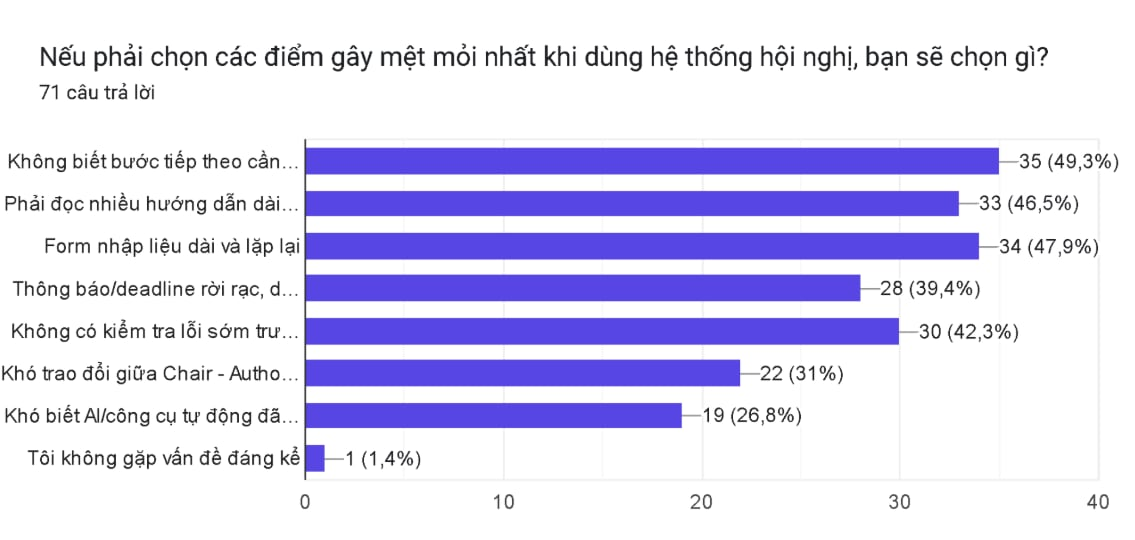
\includegraphics[width=0.9\textwidth]{images/chapter_2_picture_2.jpg}
    \caption{Các vấn đề người dùng gặp phải khi tham gia quy trình hội nghị khoa học}
    \label{fig:ch2-user-pain-points}
\end{figure}

Hình~\ref{fig:ch2-user-pain-points} minh họa phân bố các vấn đề nổi bật. Bảng dưới đây trình bày số liệu thu được từ khảo sát của nhóm.

\begin{center}
\small
\begin{tabular}{|P{0.23\textwidth}|P{0.23\textwidth}|P{0.23\textwidth}|P{0.23\textwidth}|}
\hline
Vấn đề nổi bật & Số người chọn & Tỷ lệ trên 71 phản hồi & Diễn giải thiết kế \\ \hline
Không biết bước tiếp theo cần làm là gì & 35 & 49,3\% & Hệ thống cần bảng điều khiển và lời nhắc hành động theo trạng thái, tránh để người dùng tự dò quy trình. \\ \hline
Biểu mẫu nhập liệu dài và lặp lại & 34 & 47,9\% & Quy trình nộp bài cần hỗ trợ trích xuất siêu dữ liệu từ tệp bài báo và cho phép người dùng chỉnh sửa trước khi gửi. \\ \hline
Phải đọc nhiều hướng dẫn dài trước khi thao tác & 33 & 46,5\% & Giao diện cần tổ chức thao tác theo từng bước, sử dụng ngôn ngữ rõ ràng và cung cấp trợ lý theo ngữ cảnh. \\ \hline
Không có kiểm tra lỗi sớm trước khi nộp chính thức & 30 & 42,3\% & Hệ thống cần kiểm tra sơ bộ trước khi bài nộp đi vào quy trình phản biện chính thức. \\ \hline
Thông báo và hạn chót bị phân tán, dễ bỏ sót & 28 & 39,4\% & Hệ thống cần tập trung thông báo và cập nhật trạng thái, thay vì phụ thuộc hoàn toàn vào thư điện tử. \\ \hline
\end{tabular}
\end{center}

Những số liệu này cho thấy khó khăn của người dùng không chỉ bắt nguồn từ việc thiếu chức năng nghiệp vụ. Nhiều hệ thống hiện có đã hỗ trợ nộp bài, phản biện và ra quyết định, nhưng quy trình thao tác vẫn phức tạp, phân tán và khó theo dõi. Vì vậy, ConferenceSpace không chỉ cần bao phủ các nghiệp vụ quản lý hội nghị mà còn phải giảm số bước và lượng thông tin người dùng phải nhập hoặc kiểm tra nhiều lần.

\subsection{Kết quả theo vai trò}

\subsubsection{a) Nhóm Chủ tọa/Ban tổ chức}

Trong nhóm người tham gia với vai trò Chủ tọa, các tính năng được quan tâm gồm cảnh báo xung đột lợi ích, bảng điều khiển trạng thái hội nghị và hỗ trợ phân công Phản biện viên. Tuy nhiên, số lượng Chủ tọa trong mẫu còn nhỏ nên các tỷ lệ của nhóm này chỉ có giá trị định hướng ưu tiên ban đầu.

\begin{center}
\small
\begin{tabular}{|P{0.31\textwidth}|P{0.31\textwidth}|P{0.31\textwidth}|}
\hline
Tính năng & Kết quả ghi nhận & Diễn giải \\ \hline
Cảnh báo xung đột lợi ích & 5/7 Chủ tọa đánh giá cao & Chủ tọa cần cơ chế cảnh báo sớm để tránh phân công sai người, nhưng kết quả cuối cùng vẫn cần người có thẩm quyền xác nhận. \\ \hline
Bảng điều khiển tóm tắt tình trạng hội nghị & 4/7 Chủ tọa đánh giá cao & Nhu cầu chính là giảm tải việc theo dõi thủ công qua nhiều bảng, thư điện tử và trang trạng thái rời rạc. \\ \hline
Gợi ý Phản biện viên theo chuyên môn & 2/7 Chủ tọa đánh giá cao & Tín hiệu này cho thấy Chủ tọa có thể thận trọng với việc tự động hóa phân công Phản biện viên; vì vậy, hệ thống nên trình bày gợi ý dưới dạng danh sách có điểm số và lý do rõ ràng, thay vì đưa ra quyết định tự động. \\ \hline
\end{tabular}
\end{center}

Tính năng đối sánh phản biện trong ConferenceSpace thuộc lớp thuật toán xác định, không phải luồng AI tạo sinh. Chủ tọa cần biết căn cứ xếp hạng phản biện viên, xung đột lợi ích nào đang ngăn việc phân công và có quyền ghi đè kết quả khi có căn cứ nghiệp vụ.

\subsubsection{b) Nhóm Tác giả}

Đối với Tác giả, nhu cầu nổi bật nhất là giảm lượng thông tin phải nhập trong quy trình nộp bài. Có 21 người chọn phương án ``tự điền và cho phép tôi sửa nhanh những mục sai'' cho chức năng Submission Autofill. Kết quả này cho thấy người dùng muốn hệ thống thực hiện các thao tác lặp lại nhưng không tự gửi bài thay họ; bước xác nhận vẫn thuộc trách nhiệm của Tác giả.

\begin{center}
\small
\begin{tabular}{|P{0.31\textwidth}|P{0.31\textwidth}|P{0.31\textwidth}|}
\hline
Tính năng & Kết quả ghi nhận & Diễn giải \\ \hline
Submission Autofill & Lựa chọn phổ biến nhất là tự điền nhưng cho phép sửa & Tính năng này nên tạo dữ liệu nháp, hiển thị các trường đã trích xuất và cho phép Tác giả chỉnh sửa. \\ \hline
Submission Gating & Người tham gia đánh giá tính năng này là hữu ích & Submission Gating nên cảnh báo lỗi sớm, nhưng không được tự động loại bài khi chưa có chính sách rõ ràng. \\ \hline
\end{tabular}
\end{center}

Xét về thiết kế, đây là nhóm tính năng ảnh hưởng trực tiếp nhất đến trải nghiệm ban đầu của Tác giả với hệ thống. Quy trình nộp bài cần giúp người dùng hoàn thành đúng yêu cầu, hiểu rõ trạng thái và sửa lỗi trước hạn chót.

\subsubsection{c) Nhóm Phản biện viên}

\begin{figure}[htbp]
    \centering
    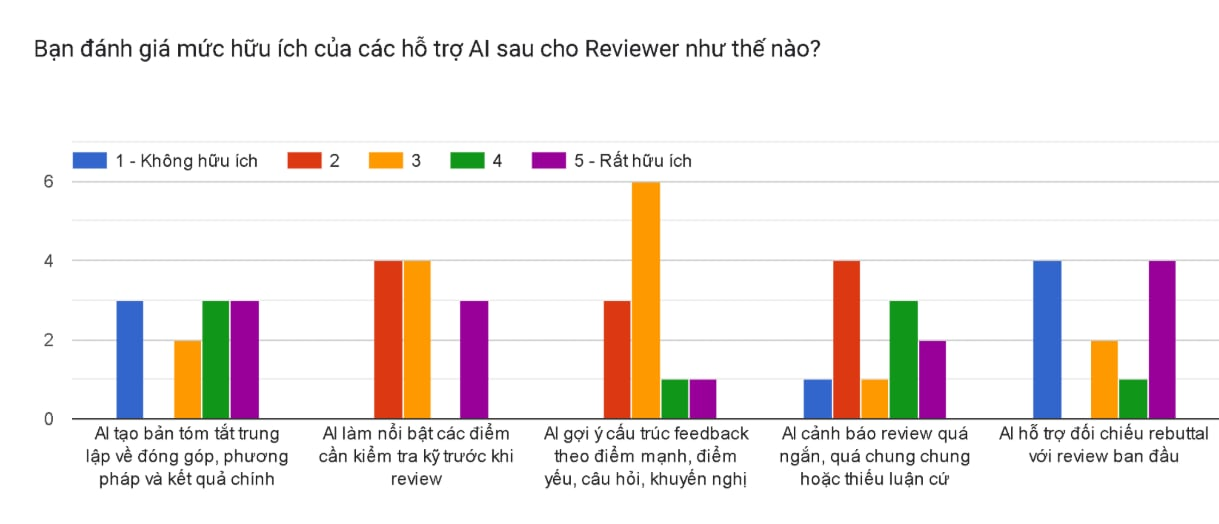
\includegraphics[width=0.9\textwidth]{images/chapter_2_picture_3.jpg}
    \caption{Mức độ ủng hộ AI của Phản biện viên theo từng tác vụ}
    \label{fig:ch2-reviewer-ai-acceptance}
\end{figure}

Hình~\ref{fig:ch2-reviewer-ai-acceptance} thể hiện mức độ chấp nhận AI của Phản biện viên theo từng tác vụ. Trong dữ liệu khảo sát, 6/11 Phản biện viên đánh giá cao tính năng dùng AI để tạo bản tóm tắt trung lập, trong khi chỉ 3/11 đánh giá cao tính năng dùng AI để nêu bật những điểm cần kiểm tra kỹ.

\begin{center}
\small
\begin{tabular}{|P{0.31\textwidth}|P{0.31\textwidth}|P{0.31\textwidth}|}
\hline
Tính năng & Kết quả ghi nhận & Diễn giải \\ \hline
Tóm tắt trung lập bài báo & 6/11 Phản biện viên đánh giá cao & AI có thể giúp Phản biện viên nắm bối cảnh ban đầu, nhưng bản tóm tắt không thay thế việc đọc bài. \\ \hline
Nêu bật điểm cần kiểm tra kỹ & 3/11 Phản biện viên đánh giá cao & Phản biện viên thận trọng với việc AI định hướng đánh giá học thuật; đầu ra nên là gợi ý kiểm tra, không phải kết luận chuyên môn. \\ \hline
\end{tabular}
\end{center}

Kết quả này phù hợp với các chính sách gần đây của những hội nghị lớn: AI có thể hỗ trợ Phản biện viên trong điều kiện được kiểm soát, nhưng Phản biện viên vẫn chịu trách nhiệm cuối cùng về nội dung bản phản biện, tính bảo mật của bản thảo và tính trung thực của đánh giá \cite{ch2ref15,ch2ref16}.

Do đó, AI chỉ nên hỗ trợ Phản biện viên định hướng việc đọc, không thay con người đọc và đánh giá bài báo. Khảo sát chưa đo khối lượng ghi chú, số lần đối chiếu hoặc thời gian rà soát; kết quả chỉ cho thấy người tham gia có xu hướng chấp nhận AI ở vai trò tạo bản tóm tắt và nêu những điểm cần kiểm tra.

\subsection{Diễn giải kết quả và giới hạn khảo sát}

Tổng hợp các phản hồi cho thấy bốn nhu cầu nền tảng:

\begin{enumerate}
    \item \textbf{Giảm thao tác thủ công:} người dùng muốn hệ thống xử lý phần nhập liệu và kiểm tra lặp lại, đặc biệt ở bước nộp bài.
    \item \textbf{Giảm tải nhận thức:} người dùng cần biết trạng thái hiện tại, việc tiếp theo cần làm và hạn chót liên quan mà không phải tự dò nhiều trang hoặc thư điện tử.
    \item \textbf{Tăng khả năng kiểm soát rủi ro:} Chủ tọa cần công cụ hỗ trợ phát hiện xung đột lợi ích và theo dõi tiến độ phản biện; Tác giả cần phát hiện lỗi trước khi gửi chính thức.
    \item \textbf{Bảo đảm tính minh bạch của AI:} người dùng chấp nhận AI khi công nghệ này chỉ đóng vai trò hỗ trợ, đưa ra kết quả có căn cứ và cho phép con người kiểm tra lại.
\end{enumerate}

Những kết luận này cần được diễn giải trong ba giới hạn. Thứ nhất, khảo sát sử dụng mẫu thuận tiện gồm 71 phản hồi nên không thể đại diện cho toàn bộ cộng đồng học thuật. Thứ hai, nhóm Chủ tọa và nhóm Phản biện viên có quy mô nhỏ; do đó, phân tích theo vai trò chỉ mang tính định hướng. Thứ ba, khảo sát này đo nhu cầu trước khi người tham gia sử dụng hệ thống, khác với khảo sát sau trải nghiệm được trình bày trong chương đánh giá.

\section{Khảo sát hiện trạng các hệ thống quản lý hội nghị}

\subsection{Đối tượng, tiêu chí và giới hạn khảo sát}

Nhóm chia các hệ thống khảo sát thành hai nhóm với mục đích đối chiếu khác nhau. Nhóm thứ nhất gồm EasyChair, HotCRP, OpenReview và Microsoft CMT. Các nền tảng này đã hoàn thiện quy trình nghiệp vụ và cung cấp chuẩn tham chiếu về vòng đời xét duyệt, vai trò, phân quyền, phân công, xung đột lợi ích, phản biện, phản hồi của tác giả và ra quyết định. Nhóm thứ hai gồm PeerSubmit, nền tảng lấy AI làm trọng tâm, và Morressier, đối tượng tham khảo bổ sung. PeerSubmit minh họa chiến lược đưa AI vào nhiều công đoạn của vòng đời; Morressier bổ sung góc nhìn về sàng lọc liêm chính, khai báo xung đột lợi ích và phân công phản biện có sự xác nhận của ban tổ chức.

Nhóm đối chiếu các nền tảng theo tám tiêu chí:

\begin{itemize}
    \item Mức bao phủ vòng đời xét duyệt và các vai trò được hỗ trợ;
    \item Các khâu tích hợp AI hoặc thuật toán trong vòng đời;
    \item Loại đầu ra được tạo và mức độ gần với quyết định học thuật;
    \item Cơ chế xác nhận, ghi đè hoặc chặn hành động;
    \item Khả năng giải thích, truy vết và kiểm tra lại kết quả;
    \item Phạm vi phân quyền đối với dữ liệu bài nộp và dữ liệu người dùng;
    \item Loại bằng chứng hỗ trợ cho từng nhận định;
    \item Các chức năng ngoài xét duyệt như đăng ký, thanh toán và trang thông tin sự kiện; tiêu chí này chỉ dùng để xác định phạm vi sản phẩm, không dùng để kết luận về chất lượng học thuật.
\end{itemize}

\subsection{Tổng quan các hệ thống hiện có}

\subsubsection{a) EasyChair}

EasyChair là hệ thống quản lý hội nghị có phạm vi sử dụng lớn theo số liệu do nhà cung cấp công bố. Trang chính thức của EasyChair nêu hơn 4,8 triệu người dùng và hơn 124.000 hội nghị đã sử dụng nền tảng này \cite{ch2ref1}. Hệ thống hỗ trợ nhiều thành phần của vòng đời hội nghị, bao gồm nộp bài, quản lý phản biện, quản lý quyền truy cập, xung đột lợi ích, phân công phản biện theo nguyện vọng, phản hồi của tác giả, thư điện tử, phân tích dữ liệu và xuất bản kỷ yếu \cite{ch2ref2}.

Bằng chứng từ cộng đồng hội nghị xác nhận EasyChair có thể vận hành một quy trình phản biện nhiều giai đoạn. ITiCSE 2025 sử dụng EasyChair cho phản biện kín hai chiều, đăng ký nguyện vọng phản biện, khai báo xung đột lợi ích, phân công bằng thuật toán, thảo luận và tổng hợp nhận xét của phản biện viên cấp cao \cite{ch2ref57}. Ở chiều ngược lại, một báo cáo kinh nghiệm công bố năm 2013 của thành viên ban tổ chức hội nghị ghi nhận rằng một số tùy chọn cấu hình khi đó khó tìm và phải thử nhiều lần mới hiểu, dù quy trình trở nên hữu ích sau khi người dùng đã làm quen \cite{ch2ref22}. Đây là một trường hợp sử dụng cụ thể, không đủ để kết luận EasyChair nhìn chung dễ hay khó sử dụng. Vì vậy, bài học phù hợp cho ConferenceSpace là tham khảo phạm vi quy trình của EasyChair, đồng thời đánh giá khả năng hướng dẫn theo ngữ cảnh bằng thử nghiệm người dùng của chính hệ thống thay vì suy diễn từ tài liệu hướng dẫn của EasyChair.

\subsubsection{b) HotCRP}

HotCRP hỗ trợ nhiều thành phần của quy trình phản biện và hoạt động điều phối của Chủ tọa. Theo tài liệu của HotCRP, hệ thống hỗ trợ phân công bài, đăng ký nguyện vọng phản biện, xung đột lợi ích, Chủ tọa ra quyết định, vai trò người điều phối thảo luận (lead), người hướng dẫn hoàn thiện bản sửa (shepherd), phân công tự động và chế độ chạy thử để kiểm tra kết quả trước khi áp dụng \cite{ch2ref3}. Tài liệu hướng dẫn dành cho Chủ tọa cũng mô tả cơ chế xử lý xung đột của Chủ tọa, quản trị viên phụ trách từng bài và có sử dụng cơ chế mã cấp quyền phản biện dùng để giới hạn quyền truy cập khi có xung đột \cite{ch2ref4}.

Báo cáo của hai đồng Chủ tọa chương trình USENIX ATC 2020 cung cấp bằng chứng vận hành cụ thể hơn. HotCRP hỗ trợ phân công hàng trăm bài cho hơn 100 thành viên ban chương trình; kết quả phân công tự động ban đầu được đánh giá là hữu ích nhưng vẫn cần Chủ tọa rà soát và điều chỉnh đáng kể. Báo cáo cũng ghi nhận danh mục chủ đề quá chi tiết làm tăng gánh nặng khai báo và có thể làm giảm chất lượng phân công ban đầu, trong khi cơ chế xung đột lợi ích ngăn thành viên có xung đột truy cập bài, điểm số và thảo luận liên quan \cite{ch2ref58}. Bằng chứng này xác nhận HotCRP đã được dùng để thực thi quy tắc truy cập và hỗ trợ Chủ tọa giám sát phân công, nhưng không chứng minh nền tảng chỉ phù hợp với người dùng có kinh nghiệm. ConferenceSpace vì vậy tham khảo nguyên tắc kiểm soát quyền và xác nhận phân công, còn mức độ dễ tiếp cận phải được đánh giá riêng trên người dùng của hệ thống.

\subsubsection{c) OpenReview}

OpenReview là nền tảng quản lý phản biện có khả năng cấu hình nhiều mức độ công khai. Trang giới thiệu chính thức mô tả đây là nền tảng đám mây cung cấp giao diện lập trình để truy cập dữ liệu theo quyền đọc và quyền ghi, hỗ trợ thảo luận mở, quản lý thông tin phục vụ xác định xung đột lợi ích và đối sánh bài báo với phản biện viên cho các hội nghị có hàng nghìn bài nộp \cite{ch2ref5}.

Các Chủ tọa chương trình NeurIPS 2021 đã chuyển toàn bộ quy trình sang OpenReview nhưng vẫn áp dụng phản biện kín hai chiều: trong thời gian xét duyệt, bài nộp chỉ hiển thị cho thành viên ban chương trình được phân công và các thảo luận nội bộ tiếp tục được giữ kín; chỉ bài được chấp nhận cùng các bản phản biện ẩn danh mới được công khai sau thời điểm thông báo \cite{ch2ref59}. Báo cáo sau hội nghị của các Chủ tọa chương trình ACT 2023 cũng cho thấy OpenReview phiên bản 1 có thể thích nghi với quy trình phản biện kín một chiều, nhưng một số xung đột lợi ích đặc thù, quyền xem thảo luận và việc thêm phản biện viên phụ vẫn cần cấu hình qua giao diện lập trình hoặc xử lý thủ công \cite{ch2ref60}. Vì vậy, điểm tham khảo có bằng chứng của OpenReview là khả năng cấu hình mức độ công khai và quyền truy cập; ConferenceSpace cần bảo đảm tính minh bạch có kiểm soát thay vì mặc định công khai toàn bộ quy trình.

\subsubsection{d) Microsoft CMT}

Microsoft CMT hỗ trợ nhiều vai trò, nhiều tiểu ban chuyên môn, toàn bộ vòng đời nộp bài, biểu mẫu tùy chỉnh, quản lý xung đột, đăng ký nguyện vọng phản biện, gợi ý phản biện viên, thảo luận, phản hồi của tác giả và phân công tích hợp với TPMS \cite{ch2ref6}. Tài liệu CMT về quản lý xung đột nêu hai cơ chế chính: xung đột theo cá nhân và xung đột theo miền thư điện tử; các xung đột này được xét trong quá trình phân công \cite{ch2ref7}. Theo tài liệu TPMS, điểm TPMS nằm trong khoảng từ 0 đến 1; điểm càng cao thì mức độ phù hợp giữa bài báo và phản biện viên càng lớn \cite{ch2ref8}.

Báo cáo của các Chủ tọa CVPR 2013 cho biết CMT đã quản lý toàn bộ quá trình nộp và xét duyệt 1.798 bài được phản biện đầy đủ. TPMS cung cấp gợi ý đối sánh; CMT chọn ba phản biện viên không có xung đột cho mỗi bài từ danh sách ứng viên; sau đó các Chủ tọa và Chủ tọa lĩnh vực vẫn thực hiện nhiều điều chỉnh thủ công để cải thiện mức độ phù hợp dưới ràng buộc về khối lượng công việc. Báo cáo kết luận trách nhiệm phân công thuộc về các Chủ tọa, còn CMT và TPMS đóng vai trò hỗ trợ \cite{ch2ref61}. Bằng chứng vận hành này củng cố cách ConferenceSpace thiết kế đối sánh như một chức năng hỗ trợ có thể kiểm tra, kết hợp điểm phù hợp chuyên môn, xung đột lợi ích, khối lượng công việc và quyền xác nhận của Chủ tọa, thay vì tự động ra quyết định cuối cùng.

\subsubsection{e) PeerSubmit: nền tảng lấy AI làm trọng tâm}

PeerSubmit tự định vị là nền tảng lấy AI làm trọng tâm trong quản lý bài nộp và xét duyệt. Tài liệu sản phẩm công bố một vòng đời chung gồm cấu hình hội nghị hoặc tạp chí, tiếp nhận bài, phân công phản biện viên, phản biện và ra quyết định. Nền tảng hỗ trợ nhiều tiểu ban chuyên môn, các chế độ phản biện kín một chiều, kín hai chiều và công khai, biểu mẫu chấm điểm, phản hồi của tác giả, nhiều vòng chỉnh sửa, phân quyền theo vai trò và nhật ký hoạt động \cite{ch2ref48}.

Danh mục chức năng AI trên trang sản phẩm gồm đối sánh phản biện theo chuyên môn kèm điểm tin cậy và kiểm tra xung đột lợi ích, tóm tắt bài nộp, sàng lọc chất lượng và mức độ phù hợp với phạm vi hội nghị, cùng bản tóm lược hỗ trợ quyết định (decision brief) tổng hợp điểm và nhận xét \cite{ch2ref48}. Bài viết kỹ thuật của nhà cung cấp mô tả phương pháp đối sánh bằng biểu diễn nhúng cho bài báo và hồ sơ phản biện viên, chỉ mục HNSW, truy vấn $K$ kết quả gần nhất, xếp hạng theo độ tương đồng cosine, sau đó lọc theo xung đột lợi ích và tình trạng sẵn sàng \cite{ch2ref53}. Đây là kiến trúc do nhà cung cấp mô tả; nguồn không công bố mô hình nhúng, dữ liệu đánh giá hoặc kết quả kiểm chứng độc lập, nên báo cáo không kết luận về việc triển khai thực tế hoặc chất lượng đối sánh.

Ranh giới trách nhiệm trong tài liệu PeerSubmit chưa hoàn toàn nhất quán. Trang sản phẩm mô tả Chủ tọa sử dụng bảng điều khiển quyết định để chấp nhận, từ chối hoặc yêu cầu sửa bài, còn bản tóm lược hỗ trợ quyết định chỉ tổng hợp điểm phản biện \cite{ch2ref48}. Bài viết về AI trong xét duyệt cũng khẳng định AI không đưa ra quyết định chấp nhận hoặc từ chối và phán đoán của con người vẫn giữ vai trò trung tâm \cite{ch2ref54}. Tuy nhiên, trang thông tin đồng thời quảng bá chức năng AI hỗ trợ chấm điểm bản phản biện và chức năng tạo phán quyết cuối cùng kèm điểm tin cậy \cite{ch2ref52}. Báo cáo xem sự khác biệt này là một giới hạn của tài liệu do nhà cung cấp công bố; nhóm không suy diễn rằng PeerSubmit hoàn toàn tự động ra quyết định, đồng thời không xem quyền ghi đè của con người là đặc điểm riêng của ConferenceSpace.

PeerSubmit tự công bố mức giảm 70\% đối với chu kỳ xét duyệt, 99\% đối với thời gian phân công và 40\% đối với thời gian phản biện, cùng tỷ lệ phù hợp giữa bài báo và phản biện viên là 96\% \cite{ch2ref48}. Trong phạm vi khảo sát, nhóm chưa tìm thấy báo cáo vận hành của một hội nghị, đánh giá cộng đồng hoặc nghiên cứu độc lập công bố dữ liệu nguồn, cỡ mẫu, tập tham chiếu, định nghĩa chỉ số và phương pháp đo tương ứng. Vì vậy, báo cáo chỉ xem các tỷ lệ này là tuyên bố của nhà cung cấp, không dùng làm kết quả thực nghiệm hoặc đường cơ sở cho ConferenceSpace. Tài liệu PeerSubmit cho thấy tự động hóa tại nhiều công đoạn là một chiến lược định vị sản phẩm. Do đó, câu hỏi có ý nghĩa đối với ConferenceSpace không còn là ``có tích hợp AI hay không'', mà là ``tác vụ nào nên dùng AI, tác vụ nào phải cho kết quả có thể tái tạo, ai xác nhận đầu ra và cần bằng chứng nào để đánh giá từng lựa chọn''.

\subsubsection{f) Morressier: tham khảo về liêm chính và phân công có xác nhận}

Morressier thể hiện một chiến lược khác: tích hợp kiểm tra đạo văn, trùng lặp hình ảnh và dấu hiệu của "cơ sở sản xuất bài báo hàng loạt" (paper mill) vào quy trình Integrity Manager để nhóm biên tập xem báo cáo trước khi ra quyết định \cite{ch2ref47}. Tài liệu Auto-Assign mô tả việc phân phối bài đều nhất có thể giữa các phản biện viên đã chấp nhận và tạo danh sách gợi ý để người tổ chức sửa trước khi xác nhận. Các điều kiện chặn được nêu cụ thể gồm phản biện viên đã được phân công cho bài, đã từ chối bài, là đồng tác giả của bài hoặc đã quá hạn phản biện \cite{ch2ref55}; phạm vi này không đủ để kết luận chức năng tự động phát hiện mọi dạng xung đột lợi ích. Từ phía cộng đồng xuất bản, IOP Publishing xác nhận đã hợp tác với Morressier để tích hợp luồng tiếp nhận, phản biện và xuất bản kỷ yếu cho các đơn vị tổ chức hội nghị mà IOP phục vụ \cite{ch2ref62}. Tuy nhiên, thông báo này được công bố năm 2021, trước khi Integrity Manager ra mắt, và không đánh giá Auto-Assign. Do đó, báo cáo chỉ dùng Morressier để tham khảo hai mẫu thiết kế cần được kiểm chứng thêm là sàng lọc liêm chính chuyên biệt và phân công có bước xác nhận, chứ không dùng làm bằng chứng về chất lượng hoặc hiệu quả của hai chức năng.

\subsection{So sánh phạm vi nghiệp vụ}

Bảng dưới đây xem xét liệu ConferenceSpace có đặt các thử nghiệm thuật toán và AI trong một vòng đời xét duyệt thống nhất hay chỉ ghép các luồng xử lý rời rạc. Mức hỗ trợ của các nền tảng đối chiếu được tổng hợp từ tài liệu công khai; cột ConferenceSpace chỉ mô tả phạm vi đề tài, không đánh giá chất lượng.

\begingroup
\small
\setlength{\tabcolsep}{2pt}
\setlength{\LTleft}{0pt}
\setlength{\LTright}{0pt}
\begin{longtable}{|P{0.17\textwidth}|P{0.20\textwidth}|P{0.20\textwidth}|P{0.20\textwidth}|P{0.17\textwidth}|}
  \caption{So sánh phạm vi nghiệp vụ của các nhóm nền tảng}\\
\hline
Nhóm nghiệp vụ & EasyChair/HotCRP & OpenReview/CMT & PeerSubmit & ConferenceSpace \\ \hline
\endfirsthead
\hline
Nhóm nghiệp vụ & EasyChair/HotCRP & OpenReview/CMT & PeerSubmit & ConferenceSpace \\ \hline
\endhead
\hline
\endfoot
Cấu hình hội nghị và chuyên đề & Có, với mức cấu hình khác nhau & Có & Có & Có trong phạm vi đề tài \\ \hline
Nộp bài, sửa bài và theo dõi trạng thái & Có & Có & Có & Có \\ \hline
Vai trò và phân quyền & Có & Có & Có, công bố cơ chế phân quyền theo vai trò & Có theo các vai trò Tác giả, Phản biện viên và Chủ tọa/Đồng chủ tọa \\ \hline
Phân công phản biện và xung đột lợi ích & Có cơ chế đăng ký nguyện vọng, ràng buộc hoặc khai báo xung đột & Có đối sánh, đăng ký nguyện vọng, TPMS và kiểm tra xung đột lợi ích & Có đối sánh kèm điểm tin cậy và kiểm tra xung đột lợi ích theo công bố của nhà cung cấp & Có thuật toán đối sánh xác định, cung cấp điểm và thông tin xung đột lợi ích để Chủ tọa xác nhận \\ \hline
Biểu mẫu, bản nháp và gửi bản phản biện & Có & Có & Có & Có \\ \hline
Phản hồi của tác giả, thảo luận và vòng chỉnh sửa & Có tùy cấu hình & Có & Có theo tài liệu sản phẩm & Có trong phạm vi luồng đã xây dựng \\ \hline
Quyết định và thông báo & Có & Có & Có bảng điều khiển quyết định và thư thông báo & Chủ tọa ra quyết định; hệ thống quản lý trạng thái và thông báo \\ \hline
Bản hoàn thiện sau chấp nhận & Có ở một số nền tảng & Có tùy quy trình & Có bước chấp nhận cuối cùng và công bố theo mô tả sản phẩm & Chỉ hỗ trợ tải lên và truy xuất tệp sau khi bài được chấp nhận; chưa có bước phê duyệt, thực thi hạn chót hoặc yêu cầu nộp lại \\ \hline
Đăng ký, thanh toán và trang thông tin sự kiện & Có ở một số gói hoặc qua tích hợp & Không phải trọng tâm chung & Có các chức năng sự kiện theo trang thông tin giá & Nằm ngoài phạm vi đề tài \\ \hline
\end{longtable}
\endgroup

Kết quả so sánh cho thấy ConferenceSpace tổ chức các thành phần nộp bài, phân công, xung đột lợi ích, phản biện, phản hồi của tác giả, ra quyết định và tải bản hoàn thiện sau chấp nhận trong cùng một mô hình trạng thái và quyền hạn. Vì vậy, các luồng hỗ trợ không phải những bản minh họa độc lập. Bảng chỉ xác nhận phạm vi đã xây dựng theo mô tả thiết kế, không xác nhận các chức năng vận hành đúng trong toàn bộ quy trình.

\subsection{So sánh với nền tảng có chiến lược lấy AI làm trọng tâm và quy ước trách nhiệm}

Bảng sau đối chiếu cách các nền tảng tích hợp cơ chế tự động hóa hoặc AI vào vòng đời xét duyệt. Mỗi ô mô tả quy ước được công bố về tác vụ, đầu ra và người xác nhận; bảng không nhằm xếp hạng chất lượng. Nội dung về PeerSubmit và Morressier dựa trên tuyên bố của nhà cung cấp, còn cột ConferenceSpace trình bày quy ước thiết kế. Mức độ triển khai và bằng chứng được đánh giá riêng ở Chương 4.

\begingroup
\small
\setlength{\tabcolsep}{2pt}
\setlength{\LTleft}{0pt}
\setlength{\LTright}{0pt}
\begin{longtable}{|P{0.16\textwidth}|P{0.24\textwidth}|P{0.27\textwidth}|P{0.27\textwidth}|}
  \caption{So sánh chiến lược AI và quy ước trách nhiệm}\\
\hline
Tác vụ & Nền tảng đã hoàn thiện nghiệp vụ/Morressier & PeerSubmit theo tài liệu nhà cung cấp & ConferenceSpace \\ \hline
\endfirsthead
\hline
Tác vụ & Nền tảng đã hoàn thiện nghiệp vụ/Morressier & PeerSubmit theo tài liệu nhà cung cấp & ConferenceSpace \\ \hline
\endhead
\hline
\endfoot
Nhập liệu và sàng lọc & Các nền tảng đã hoàn thiện nghiệp vụ sử dụng biểu mẫu; Morressier công bố chức năng kiểm tra trước khi nộp và kiểm tra liêm chính chuyên biệt & Công bố chức năng sàng lọc chất lượng và mức độ phù hợp với phạm vi hội nghị, trích xuất chủ đề và từ khóa & Submission Autofill tạo bản nháp để Tác giả sửa và xác nhận; Submission Gating tách lỗi theo quy tắc khỏi cảnh báo về nội dung do AI phát hiện \\ \hline
Đối sánh phản biện & CMT sử dụng TPMS; Morressier phân công tự động theo chủ đề, tải và xung đột, sau đó người tổ chức xác nhận & Sử dụng biểu diễn nhúng, HNSW, truy vấn $K$ kết quả gần nhất, độ tương đồng cosin và bộ lọc xung đột lợi ích; Chủ tọa có thể phê duyệt hoặc ghi đè gợi ý & Sử dụng Jaccard cùng ràng buộc về khối lượng công việc và xung đột lợi ích để cho kết quả xác định; Chủ tọa xác nhận hoặc ghi đè quyết định \\ \hline
Phát hiện xung đột lợi ích & Nhiều nền tảng có cơ chế khai báo hoặc quy tắc xung đột; Morressier chặn một số trường hợp phân công & Công bố chức năng tự động kiểm tra xung đột lợi ích trong quá trình đối sánh & Kết hợp tự kiểm tra, khai báo và đồ thị đồng tác giả; hiển thị bằng chứng nhưng không tuyên bố phát hiện đầy đủ \\ \hline
Tóm tắt bài nộp & Không phải năng lực cốt lõi chung của nhóm nền tảng đã hoàn thiện nghiệp vụ & Công bố chức năng tóm tắt phương pháp, đóng góp và cảnh báo các vấn đề về chất lượng & Reviewer Initial Analysis tạo bản tóm tắt, nêu điểm mạnh, điểm yếu, gợi ý; không tự điền, gửi, chấm điểm hoặc đưa ra khuyến nghị cuối cùng trong biểu mẫu phản biện \\ \hline
Rà soát bản phản biện & Sử dụng biểu mẫu và quy tắc nghiệp vụ; Morressier tập trung vào tính liêm chính của bài nộp & Trang thông tin giá công bố chức năng AI hỗ trợ chấm điểm bản phản biện và phát hiện nội dung không nhất quán & Review Quality Auditor rà soát bản phản biện nháp trước khi gửi để  \\ \hline
Tổng hợp thông tin trước quyết định & Cung cấp bảng điểm, thảo luận và chức năng ra quyết định của Chủ tọa tùy nền tảng & Công bố bản tóm lược hỗ trợ quyết định; trang thông tin giá còn quảng bá chức năng tạo phán quyết cuối cùng, trong khi bài viết khác vẫn giao quyền chấp nhận hoặc từ chối cho con người & Chair Decision Copilot tổng hợp bằng chứng và bất đồng; chức năng này không tạo phán quyết chấp nhận hoặc từ chối bài báo \\ \hline
Trợ lý cho nhiều vai trò & Chưa ghi nhận đây là năng lực cốt lõi chung & Chưa đủ tài liệu công khai để kết luận về quy ước truy cập tài nguyên theo từng vai trò & Chatbot Agent chỉ gọi công cụ trong phạm vi quyền và từ chối yêu cầu ngoài phạm vi, ngoài quyền truy cập \\ \hline
Loại bằng chứng & Tài liệu sản phẩm và hỗ trợ; một số cơ chế có nghiên cứu riêng & Chủ yếu là tài liệu và số liệu do nhà cung cấp công bố; nhóm chưa xác nhận được đánh giá độc lập & Mã nguồn, kết quả kiểm thử, đánh giá theo tác vụ và kiểm thử chấp nhận của người dùng ở Chương 4; mức độ bằng chứng khác nhau giữa các luồng \\ \hline
\end{longtable}
\endgroup


\subsection{Đối chiếu kết quả khảo sát với bằng chứng bên ngoài và chính sách học thuật}

Khảo sát nhu cầu sử dụng mẫu thuận tiện, trong đó số người tham gia với vai trò Chủ tọa và Phản biện viên còn nhỏ. Vì vậy, nhóm đối chiếu các nguyên tắc rút ra từ khảo sát với nguồn bên ngoài để kiểm tra tính phù hợp với thực tiễn vận hành và chính sách học thuật. Bước đối chiếu này không nhằm ước lượng tỷ lệ nhu cầu trong toàn bộ cộng đồng, xác lập khoảng trống thị trường hoặc chứng minh hiệu quả của ConferenceSpace.

Nhóm phân biệt bốn loại nguồn theo phạm vi có thể kết luận. Tài liệu sản phẩm chỉ xác nhận chức năng được công bố; báo cáo của Chủ tọa hoặc ban chương trình cung cấp bằng chứng về cách một hội nghị cụ thể đã vận hành; chính sách của hội nghị, hiệp hội và nhà xuất bản xác định trách nhiệm cùng giới hạn sử dụng AI; nghiên cứu có công bố phương pháp cung cấp bằng chứng thực nghiệm trong phạm vi mẫu và thiết kế nghiên cứu. Nhóm ưu tiên nguồn chính thức và nghiên cứu gốc, đồng thời giữ lại các trường hợp khác biệt giữa chính sách thay vì xem một quy định đơn lẻ là đồng thuận của toàn cộng đồng.

Đối với phân công phản biện, các báo cáo vận hành củng cố yêu cầu kết hợp thuật toán với quyền kiểm soát của con người. Tại USENIX ATC 2020, kết quả phân công ban đầu của HotCRP được các đồng Chủ tọa đánh giá là hữu ích nhưng vẫn cần rà soát và điều chỉnh đáng kể \cite{ch2ref58}. Tại CVPR 2013, TPMS cung cấp kết quả đối sánh, CMT chọn các Phản biện viên không có xung đột từ danh sách ứng viên, sau đó Chủ tọa và Chủ tọa lĩnh vực tiếp tục điều chỉnh dưới ràng buộc về khối lượng công việc \cite{ch2ref61}. Hai trường hợp không chứng minh một thuật toán cụ thể tốt hơn các phương pháp khác, nhưng xác nhận rằng điểm phù hợp, xung đột lợi ích, khối lượng công việc và bước xác nhận là các thành phần riêng biệt của quy trình phân công.

Yêu cầu phát hiện xung đột lợi ích qua nhiều nguồn cũng phù hợp với chính sách học thuật. ACM quy định người tham gia phải khai báo xung đột tiềm ẩn, nhưng đồng thời nhấn mạnh một chính sách đáng tin cậy không thể chỉ dựa vào việc mỗi cá nhân tự xác định xung đột của mình; người phụ trách như Chủ tọa hoặc biên tập viên vẫn phải đánh giá và xử lý trường hợp được báo cáo \cite{ch2ref12}. Do đó, kết quả từ quy tắc, đồ thị đồng tác giả hoặc dữ liệu học thuật bên ngoài trong ConferenceSpace chỉ nên được trình bày như bằng chứng hỗ trợ để Chủ tọa xem xét, không phải kết luận tự động rằng một cặp bài báo-Phản biện viên chắc chắn có hoặc không có xung đột.

Nhu cầu kiểm tra liêm chính có bằng chứng khảo sát bên ngoài, nhưng phạm vi trách nhiệm còn chưa thống nhất. Nghiên cứu của Calamur và Ghosh phân tích khảo sát năm 2022 với 852 người tham gia; sau khi loại 22 người không đồng ý tham gia và 145 người không trả lời câu hỏi nào, phân tích còn 685 phiếu có dữ liệu. Trong 401 người từng thực hiện phản biện, 174 người (43,39\%) cho biết đã gặp bản thảo bị nghi ngờ vi phạm liêm chính; 540 người trong mẫu phân tích (78,83\%) kỳ vọng quy trình phản biện có khả năng nhận diện đạo văn \cite{ch2ref56}. Các tác giả đồng thời đặt vấn đề liệu trách nhiệm này thuộc về Phản biện viên, nhóm biên tập hay công cụ chuyên biệt. Vì vậy, các tỷ lệ trên củng cố nhu cầu có bước sàng lọc và chuyển bằng chứng cho người có thẩm quyền, nhưng không chứng minh AI có thể tự xác định hành vi vi phạm.

Các chính sách AI được khảo sát hội tụ ở hai yêu cầu: bảo mật bản thảo và giữ trách nhiệm ở con người; tuy nhiên, phạm vi sử dụng được phép khác nhau đáng kể. ICLR 2026 cho phép dùng mô hình ngôn ngữ lớn để cải thiện ngữ pháp và độ rõ của bản phản biện nếu khai báo, nhưng Phản biện viên vẫn chịu trách nhiệm về nội dung và không được vi phạm tính bảo mật của bài chưa công bố \cite{ch2ref15}. Ngược lại, ICML 2025 cấm Phản biện viên dùng AI tạo sinh để viết bản phản biện hoặc đưa bất kỳ nội dung nào của bài nộp hay bản phản biện vào công cụ AI tạo sinh \cite{ch2ref16}. ACM cho phép dùng công cụ để cải thiện văn bản do Phản biện viên viết nếu trước đó đã loại toàn bộ thông tin có thể nhận diện bài nộp, Tác giả và Phản biện viên. ACM cũng cho phép dùng hệ thống có cam kết duy trì tính bảo mật của thông tin được tải lên; trong cả hai trường hợp, Phản biện viên vẫn chịu trách nhiệm về thiên lệch và nội dung được tạo \cite{ch2ref40}. Nature Portfolio yêu cầu Phản biện viên không tải bản thảo lên công cụ AI tạo sinh và phải khai báo nếu AI hỗ trợ bất kỳ phần nào của việc đánh giá các tuyên bố trong bài \cite{ch2ref41}. Sự khác biệt này cho thấy chức năng AI cho Phản biện viên phải có khả năng bật, tắt hoặc giới hạn theo chính sách của từng hội nghị; một cấu hình chung không thể mặc nhiên phù hợp với mọi nơi.

Bằng chứng thực nghiệm hiện có cũng ủng hộ cách tiếp cận thử nghiệm có kiểm soát thay vì giả định AI luôn cải thiện phản biện. Tại ICLR 2025, Review Feedback Agent chỉ cung cấp góp ý tùy chọn trên bản phản biện do con người đã viết và không trực tiếp sửa nội dung. Trong thử nghiệm ngẫu nhiên quy mô lớn, 26,6\% Phản biện viên nhận góp ý đã cập nhật bản phản biện; nhóm nghiên cứu còn báo cáo bản phản biện được sửa dài hơn và được đánh giá cao hơn trong phép đánh giá mù, nhưng thừa nhận cần tiếp tục nghiên cứu giới hạn của phản hồi do AI tạo \cite{ch2ref17,ch2ref18}. NeurIPS 2026 tiếp tục khảo sát một phạm vi rộng hơn bằng thử nghiệm tự nguyện: Tác giả và Phản biện viên phải đồng ý tham gia, các phân công được chia ngẫu nhiên giữa điều kiện không dùng AI và hai điều kiện hỗ trợ, dữ liệu không được nhà cung cấp lưu giữ, còn Chủ tọa lĩnh vực đánh giá bản phản biện mà không biết điều kiện thử nghiệm. Công cụ được định vị để hỗ trợ hiểu và phân tích bài, không viết bản phản biện hoặc thay thế phán đoán của Phản biện viên \cite{ch2ref19}. Vì thử nghiệm NeurIPS chưa công bố kết quả tại thời điểm khảo sát, báo cáo chỉ dùng thiết kế này làm tham chiếu về biện pháp kiểm soát, không dùng làm bằng chứng về hiệu quả.

Việc đối chiếu vì vậy củng cố ba yêu cầu cho ConferenceSpace: phân công và phát hiện xung đột lợi ích phải cung cấp căn cứ để Chủ tọa xác nhận; chức năng AI phải tuân theo chính sách bảo mật và trách nhiệm của từng hội nghị; hiệu quả của mỗi luồng AI phải được đo riêng trong điều kiện sử dụng xác định. Các nhu cầu về giảm nhập liệu, chỉ dẫn bước tiếp theo và thông báo tập trung vẫn chủ yếu bắt nguồn từ khảo sát nội bộ và không được khái quát bằng các nguồn bên ngoài nêu trên. Chương 4 đánh giá mức độ đáp ứng của ConferenceSpace trong phạm vi dữ liệu, phép thử và kiểm thử chấp nhận của người dùng đã thực hiện.

\section{Vấn đề thực tiễn và nguyên tắc giải pháp}

\subsection{Các vấn đề thiết kế rút ra từ khảo sát}

Các nền tảng đã hoàn thiện phần lớn nghiệp vụ cốt lõi, còn PeerSubmit và Morressier cho thấy AI hoặc cơ chế tự động hóa đã xuất hiện ở nhiều công đoạn. Vì vậy, vấn đề của đề tài không còn là thị trường ``thiếu AI tích hợp'', mà là cách xử lý các tác vụ khác nhau về mức độ nghiêm trọng của hậu quả, yêu cầu đối với tính ổn định và chủ thể chịu trách nhiệm. Từ đó, nhóm xác định năm vấn đề thiết kế.

\textbf{Thứ nhất, giảm nhập liệu không được loại bỏ bước xác nhận của Tác giả.} Gần một nửa số người tham gia khảo sát chọn biểu mẫu dài và lặp lại là vấn đề nổi bật. Submission Autofill có thể tạo siêu dữ liệu nháp, nhưng Tác giả phải có quyền sửa từng trường và quyết định thời điểm gửi bài.

\textbf{Thứ hai, đối sánh phản biện và phát hiện xung đột lợi ích cần cho kết quả ổn định, có căn cứ.} TPMS, PeerSubmit và Morressier cho thấy nhiều chiến lược đối sánh đã được triển khai \cite{ch2ref8,ch2ref53,ch2ref55}. Tuy nhiên, phân công sai có thể ảnh hưởng đến tính công bằng và bảo mật. Vì vậy, ConferenceSpace sử dụng thuật toán xác định, hiển thị điểm số, lý do và ràng buộc, sau đó để Chủ tọa xác nhận. Lựa chọn này không hàm ý Domain Jaccard tốt hơn phương pháp đối sánh theo ngữ nghĩa.

\textbf{Thứ ba, nội dung hỗ trợ đọc và tổng hợp phải bám sát bằng chứng, đồng thời đi kèm phân tích.} Tóm tắt, cảnh báo hoặc nội dung tổng hợp có thể giảm tải nhận thức, nhưng đầu ra không cố định có thể bỏ sót thông tin, suy diễn thiếu căn cứ hoặc gây nhiễu. Mỗi luồng cần được đánh giá bằng chỉ số riêng, có phân tích các trường hợp sai và chỉ được kết luận trong phạm vi dữ liệu đã đo.

\textbf{Thứ tư, các luồng xử lý gần bước ra quyết định phải công khai mức độ ảnh hưởng đến quyền tác giả của Phản biện viên và phán quyết học thuật.} Chính sách ICLR yêu cầu người tham gia chịu trách nhiệm về nội dung của mình; ICML cấm Phản biện viên dùng AI tạo sinh để viết bản phản biện hoặc đưa nội dung mật vào công cụ AI \cite{ch2ref15,ch2ref16}. Nghiên cứu Review Feedback Agent chỉ hỗ trợ góp ý trên bản nháp do con người viết \cite{ch2ref17,ch2ref18}. ConferenceSpace không cho phép AI tự điền hoặc gửi biểu mẫu, chấm điểm hay tạo phán quyết chấp nhận hoặc từ chối.

\textbf{Thứ năm, trợ lý phục vụ nhiều vai trò phải giữ đúng ranh giới truy cập tài nguyên.} Chatbot Agent chỉ được truy vấn dữ liệu mà người dùng hiện tại có quyền xem; hệ thống phải từ chối yêu cầu ngoài phạm vi thay vì trả lời bằng suy đoán. Cơ chế phân quyền ở cấp ứng dụng không có nghĩa là hệ thống đã kiểm toán toàn bộ vòng đời lưu giữ, sử dụng để huấn luyện hoặc vị trí lưu trữ dữ liệu của nhà cung cấp AI.

Mô hình ba lớp là lựa chọn thiết kế để xử lý năm vấn đề trên: lớp nghiệp vụ cốt lõi quản lý trạng thái và quyền hạn; lớp thuật toán xác định và có thể kiểm chứng xử lý đối sánh, xung đột lợi ích và các quy tắc; lớp AI hỗ trợ có kiểm soát tạo bản nháp, phân tích, cảnh báo hoặc tổng hợp. Báo cáo không xem mô hình này là điểm mới của thị trường hay kiến trúc tối ưu duy nhất.

\subsection{Liên kết vấn đề với định hướng giải pháp}

ConferenceSpace được thiết kế để xử lý năm vấn đề trên trong phạm vi một vòng đời xét duyệt chung. Bảng sau liên kết từng vấn đề với chức năng liên quan và ranh giới trách nhiệm; mối liên kết này giải thích lựa chọn thiết kế, không thay thế bằng chứng đánh giá ở Chương 4.

\begingroup
\small
\setlength{\tabcolsep}{2pt}
\setlength{\LTleft}{0pt}
\setlength{\LTright}{0pt}
\begin{longtable}{|P{0.31\textwidth}|P{0.31\textwidth}|P{0.31\textwidth}|}
  \caption{Liên kết vấn đề thiết kế với định hướng giải pháp ConferenceSpace}\\
\hline
Vấn đề thiết kế & Định hướng trong ConferenceSpace & Ranh giới trách nhiệm \\ \hline
\endfirsthead
\hline
Vấn đề thiết kế & Định hướng trong ConferenceSpace & Ranh giới trách nhiệm \\ \hline
\endhead
\hline
\endfoot
Nộp bài thủ công, biểu mẫu dài & Submission Autofill trích xuất siêu dữ liệu từ tệp PDF và gợi ý chuyên đề trong phạm vi hội nghị & Đầu ra là bản nháp có thể chỉnh sửa; Tác giả xác nhận trước khi gửi \\ \hline
Thiếu kiểm tra lỗi sớm & Submission Gating kiểm tra các điều kiện cơ bản trước khi bài nộp đi vào quy trình phản biện & Cảnh báo hoặc chặn theo chính sách đã cấu hình; không tự động loại bài ngoài các quy tắc của hệ thống \\ \hline
Khó kiểm soát việc đối sánh phản biện và xung đột lợi ích & Thuật toán đối sánh cung cấp điểm số và kết hợp nhiều lớp phát hiện xung đột lợi ích & Đối sánh phản biện thuộc lớp thuật toán xác định; Chủ tọa ra quyết định cuối cùng \\ \hline
Phản biện viên thiếu công cụ hỗ trợ đọc hiểu ban đầu và phải tự ghi chú nhiều điểm cần kiểm tra & Reviewer Initial Analysis cung cấp bản tóm tắt, các điểm cần kiểm tra và căn cứ liên quan & AI hỗ trợ định hướng đọc; khảo sát chưa đo mức giảm thao tác, thời gian rà soát hoặc ảnh hưởng đến đánh giá chuyên môn \\ \hline
Phản biện viên cần hỗ trợ rà soát bản nháp; Chủ tọa khó tổng hợp nhiều bản phản biện và phản hồi của tác giả & Review Quality Auditor cảnh báo vấn đề trong bản nháp; Chair Decision Copilot tổng hợp điểm đồng thuận, bất đồng và rủi ro & Không tự động sửa hoặc gửi bản phản biện, cũng không tạo quyết định chấp nhận hoặc từ chối; chỉ cung cấp thông tin để người có thẩm quyền xem xét \\ \hline
Người dùng khó tìm hướng dẫn thao tác & Chatbot Agent truy vấn dữ liệu hệ thống trong phạm vi quyền truy cập & Câu trả lời phải bám dữ liệu hệ thống và không vượt quá quyền của người dùng \\ \hline
Thông báo và trạng thái phân tán & Bảng điều khiển và thông báo trong hệ thống & Tập trung trạng thái và giảm phụ thuộc vào thư điện tử \\ \hline
\end{longtable}
\endgroup

Mối liên hệ này ngăn các chức năng AI trở thành phần bổ sung không gắn với nhu cầu. Trong ConferenceSpace, mỗi luồng AI phải xử lý một vấn đề cụ thể, dừng trước hành động thuộc trách nhiệm con người và được đánh giá riêng ở Chương 4.

\subsection{Nguyên tắc thiết kế từ các vấn đề đã xác định}

Từ phân tích trên, nhóm xác định bốn nguyên tắc thiết kế cho ConferenceSpace.

\textbf{Nguyên tắc 1: Tách lớp nghiệp vụ cốt lõi, thuật toán xác định và AI hỗ trợ.} Hệ thống không giao các hoạt động nộp bài, phân công, phản biện và ra quyết định cho AI tạo sinh. Đối sánh phản biện và phát hiện xung đột lợi ích thuộc lớp thuật toán xác định vì cần bảo đảm tính nhất quán, khả năng giải thích và khả năng kiểm tra. AI chỉ tham gia các tác vụ trích xuất, tóm tắt, rà soát và tổng hợp. Thiết kế cung cấp luồng thao tác thủ công khi không dùng AI.

\textbf{Nguyên tắc 2: Con người giữ quyền quyết định học thuật và quyền thực hiện hành động nghiệp vụ.} AI không quyết định chấp nhận hay từ chối bài, không tự phân công Phản biện viên và không chấm điểm thay Phản biện viên. Kết quả do AI tạo chỉ được dùng để cảnh báo; chỉ các quy tắc xác định đối với trường bắt buộc hoặc trạng thái nghiệp vụ mới được phép chặn thao tác. Review Quality Auditor hiện chưa tuân thủ phần sau của nguyên tắc này vì kết quả cảnh báo nghiêm trọng có thể ngăn thao tác gửi nhưng chưa cho phép người dùng ghi đè. Chương 4 phải đánh giá ranh giới này là chưa đáp ứng, thay vì xem đây là cơ chế kiểm soát hoàn thiện của con người.

\textbf{Nguyên tắc 3: Mọi gợi ý quan trọng cần có căn cứ.} Gợi ý Phản biện viên cần kèm điểm phù hợp và lý do; cảnh báo xung đột lợi ích cần nêu quan hệ hoặc nguồn dữ liệu; Chair Decision Copilot cần chỉ ra bản phản biện hoặc phản hồi nào là căn cứ của nhận định tổng hợp. Đây là điều kiện để người dùng có thể đánh giá, kiểm tra và ghi đè kết quả.

\textbf{Nguyên tắc 4: Đánh giá AI theo đúng bản chất từng luồng xử lý.} Các luồng tạo dữ liệu nháp, kiểm tra sơ bộ, hỗ trợ đọc hiểu và tổng hợp bằng chứng cần được đánh giá bằng tiêu chí khác nhau. Nguyên tắc này giúp chương đánh giá về sau tránh dùng một thước đo chung cho mọi đầu ra AI hoặc diễn giải quá mức vai trò của hệ thống.

\section{Tổng hợp yêu cầu hệ thống từ khảo sát}

Mục 2.4 chuyển kết quả khảo sát và các vấn đề thiết kế thành yêu cầu hệ thống. Đây là điểm nối giữa Chương 2 và Chương 3: mỗi nhóm yêu cầu dưới đây bắt nguồn từ nhu cầu người dùng, chuẩn nghiệp vụ, xu hướng lấy AI làm trọng tâm hoặc nguyên tắc trách nhiệm đã phân tích ở trên.

\subsection{Yêu cầu chức năng theo vai trò}

\subsubsection{a) Yêu cầu cho Tác giả}

\begingroup
\small
\setlength{\tabcolsep}{2pt}
\setlength{\LTleft}{0pt}
\setlength{\LTright}{0pt}
\begin{longtable}{|P{0.31\textwidth}|P{0.31\textwidth}|P{0.31\textwidth}|}
  \caption{Yêu cầu chức năng dành cho Tác giả}\\
\hline
Mã & Yêu cầu & Cơ sở \\ \hline
\endfirsthead
\hline
Mã & Yêu cầu & Cơ sở \\ \hline
\endhead
\hline
\endfoot
F-AUTHOR-01 & Tác giả có thể tìm kiếm và xem thông tin về hội nghị, chuyên đề, hạn chót và lời mời nộp bài (CFP). & Nhu cầu theo dõi tập trung hạn chót và trạng thái. \\ \hline
F-AUTHOR-02 & Tác giả có thể nộp bài theo quy trình nhiều bước gồm khai báo thông tin bài báo, tác giả, tệp, xung đột lợi ích, xem lại và gửi. & Các hệ thống hiện có đều chuẩn hóa vòng đời nộp bài; ConferenceSpace cần bao phủ nghiệp vụ cốt lõi. \\ \hline
F-AUTHOR-03 & Submission Autofill hỗ trợ trích xuất siêu dữ liệu từ bản thảo PDF, gồm tiêu đề, tóm tắt, tác giả, cơ quan công tác, địa chỉ thư điện tử và từ khóa khi có thể. & Vấn đề nổi bật là biểu mẫu nhập liệu dài và lặp lại. \\ \hline
F-AUTHOR-04 & Submission Autofill gợi ý chuyên đề dựa trên danh sách chuyên đề đang hoạt động của hội nghị và siêu dữ liệu bài nộp. & Nhu cầu giảm thao tác chọn chuyên đề; gợi ý này hiện là một đầu ra của Submission Autofill. \\ \hline
F-AUTHOR-05 & Hệ thống kiểm tra sơ bộ bài nộp trước khi gửi chính thức và hiển thị các lỗi hoặc cảnh báo mà Tác giả có thể xử lý. & Vấn đề nổi bật là thiếu kiểm tra lỗi sớm. \\ \hline
F-AUTHOR-06 & Tác giả có thể lưu bản nháp, chỉnh sửa trước hạn chót, rút bài, xem bản phản biện, gửi phản hồi và tải bản hoàn thiện sau khi bài được chấp nhận. Luồng xử lý bản hoàn thiện chưa có bước phê duyệt, thực thi hạn chót hoặc yêu cầu nộp lại. & Yêu cầu nghiệp vụ của vòng đời xét duyệt; chức năng xử lý bản hoàn thiện mới được xây dựng một phần. \\ \hline
\end{longtable}
\endgroup

\subsubsection{b) Yêu cầu cho Phản biện viên}

\begin{table}[H]
\centering
\caption{Yêu cầu chức năng dành cho Phản biện viên}
\small
\begin{tabular}{|P{0.31\textwidth}|P{0.31\textwidth}|P{0.31\textwidth}|}
\hline
Mã & Yêu cầu & Cơ sở \\ \hline
F-REVIEWER-01 & Phản biện viên có thể chấp nhận hoặc từ chối lời mời và xem danh sách bài được phân công. & Nghiệp vụ phản biện cơ bản. \\ \hline
F-REVIEWER-02 & Phản biện viên có thể xem bài báo, tệp, siêu dữ liệu, hạn chót và trạng thái phản biện. & Nhu cầu biết rõ bước tiếp theo trong quy trình. \\ \hline
F-REVIEWER-03 & Phản biện viên có thể nhập điểm, nhận xét và mức độ tự tin, đồng thời lưu bản nháp và gửi bản phản biện chính thức. & Nghiệp vụ phản biện. \\ \hline
F-REVIEWER-04 & Hệ thống có thể cung cấp bản tóm tắt, các điểm cần kiểm tra và căn cứ liên quan để hỗ trợ bước đọc ban đầu. & Phản biện viên trong khảo sát có xu hướng chấp nhận AI ở vai trò hỗ trợ đọc; khảo sát chưa đo mức giảm thao tác hoặc thời gian rà soát. \\ \hline
F-REVIEWER-05 & AI không tự điền hoặc gửi biểu mẫu, chấm điểm hay đưa ra khuyến nghị cuối cùng. Reviewer Initial Analysis vẫn tạo nội dung có thể ảnh hưởng đến nhận định và chỉ được bật khi chính sách hội nghị cho phép. & Giới hạn các hành động thuộc trách nhiệm của Phản biện viên và công khai giới hạn chính sách của nội dung hỗ trợ \cite{ch2ref15,ch2ref16}. \\ \hline
\end{tabular}
\end{table}

\subsubsection{c) Yêu cầu cho Chủ tọa/Ban tổ chức}

\begingroup
\small
\setlength{\tabcolsep}{2pt}
\setlength{\LTleft}{0pt}
\setlength{\LTright}{0pt}
\begin{longtable}{|P{0.31\textwidth}|P{0.31\textwidth}|P{0.31\textwidth}|}
  \caption{Yêu cầu chức năng dành cho Chủ tọa và Ban tổ chức}\\
\hline
Mã & Yêu cầu & Cơ sở \\ \hline
\endfirsthead
\hline
Mã & Yêu cầu & Cơ sở \\ \hline
\endhead
\hline
\endfoot
F-CHAIR-01 & Chủ tọa có thể tạo và cấu hình hội nghị, chuyên đề, hạn chót, biểu mẫu phản biện, hội đồng chương trình và chính sách. & Nghiệp vụ cốt lõi của EasyChair, CMT và OpenReview. \\ \hline
F-CHAIR-02 & Chủ tọa có bảng điều khiển để theo dõi số bài nộp, tiến độ phản biện, hạn chót, xung đột lợi ích và các công việc cần xử lý. & Nhu cầu khắc phục tình trạng thông báo và hạn chót rời rạc; bảng điều khiển cũng được nhóm Chủ tọa quan tâm. \\ \hline
F-CHAIR-03 & Hệ thống gợi ý Phản biện viên bằng thuật toán xác định, đồng thời hiển thị điểm phù hợp, lý do và các ràng buộc. & Phân công phản biện là tác vụ quan trọng, chịu ràng buộc về tải phản biện và xung đột lợi ích \cite{ch2ref11}. \\ \hline
F-CHAIR-04 & Hệ thống phát hiện xung đột lợi ích qua nhiều lớp: trường hợp tự phản biện, khai báo thủ công, đồ thị đồng tác giả và dữ liệu học thuật bên ngoài khi phù hợp. & Không nên chỉ dựa vào khai báo của người dùng để phát hiện xung đột lợi ích \cite{ch2ref12}; dữ liệu từ các nguồn như Semantic Scholar Academic Graph API có thể bổ sung hồ sơ học thuật nhưng không thay thế bước xác nhận của Chủ tọa \cite{ch2ref13}. \\ \hline
F-CHAIR-05 & Chủ tọa có thể phân công thủ công, chấp nhận hoặc ghi đè gợi ý và theo dõi tiến độ phản biện. & Con người giữ quyền quyết định cuối cùng. \\ \hline
F-CHAIR-06 & Hệ thống hỗ trợ rà soát các bản phản biện thiếu căn cứ, quá ngắn hoặc có điểm số mâu thuẫn với nhận xét. & Nhu cầu kiểm soát chất lượng bản phản biện trong bối cảnh quá tải. \\ \hline
F-CHAIR-07 & Chair Decision Copilot chỉ tổng hợp bằng chứng, điểm đồng thuận, bất đồng, vấn đề còn bỏ ngỏ và câu hỏi cần xem xét. & Không để AI trở thành cơ chế phân loại bài được chấp nhận hay từ chối. \\ \hline
\end{longtable}
\endgroup

\subsubsection{d) Yêu cầu chung}

\begin{center}
\small
\begin{tabular}{|P{0.31\textwidth}|P{0.31\textwidth}|P{0.31\textwidth}|}
\hline
Mã & Yêu cầu & Cơ sở \\ \hline
F-COMMON-01 & Người dùng có thể sử dụng Chatbot Agent để được hỗ trợ thao tác theo ngữ cảnh và trong phạm vi quyền truy cập. & Vấn đề nổi bật là phải đọc hướng dẫn dài và không biết bước tiếp theo. \\ \hline
F-COMMON-02 & Hệ thống cung cấp thông báo trong ứng dụng và cập nhật trạng thái kịp thời. & Vấn đề nổi bật là hạn chót và thông báo bị phân tán. \\ \hline
F-COMMON-03 & Hệ thống phân quyền theo vai trò và ngăn người dùng truy cập dữ liệu ngoài phạm vi được cấp. & Yêu cầu bảo mật bản thảo và quyền riêng tư trong quy trình bình duyệt học thuật. \\ \hline
\end{tabular}
\end{center}

\subsection{Yêu cầu phi chức năng}

\begingroup
\small
\setlength{\tabcolsep}{2pt}
\setlength{\LTleft}{0pt}
\setlength{\LTright}{0pt}
\begin{longtable}{|P{0.31\textwidth}|P{0.63\textwidth}|}
  \caption{Yêu cầu phi chức năng của ConferenceSpace}\\
\hline
Nhóm yêu cầu & Nội dung \\ \hline
\endfirsthead
\hline
Nhóm yêu cầu & Nội dung \\ \hline
\endhead
\hline
\endfoot
Giảm phụ thuộc vào AI & Các thao tác nghiệp vụ cốt lõi cần có luồng thực hiện không phụ thuộc vào đầu ra AI; Chương 4 phải nêu rõ rằng khả năng cô lập lỗi đầu cuối chưa được kiểm chứng nếu chưa có thử nghiệm tương ứng. \\ \hline
Hiệu năng & Các giao diện lập trình nghiệp vụ thông thường cần phản hồi trong khoảng thời gian phù hợp với thao tác tương tác; những luồng AI có thời gian xử lý dài cần được xác định rõ là chạy đồng bộ hay chạy nền. \\ \hline
Bảo mật và dữ liệu & Hệ thống cần sử dụng HTTPS/TLS, xác thực và phân quyền theo vai trò, bảo vệ tệp bản thảo, đồng thời không đưa dữ liệu ngoài quyền truy cập vào Chatbot Agent hoặc các luồng AI. Yêu cầu này chỉ bao phủ cơ chế kiểm soát ở cấp ứng dụng; chính sách lưu giữ, sử dụng dữ liệu để huấn luyện và vị trí lưu trữ dữ liệu của nhà cung cấp cần được đánh giá riêng. \\ \hline
Khả năng giải thích & Gợi ý Phản biện viên, cảnh báo xung đột lợi ích và nội dung tổng hợp của AI cần hiển thị đủ căn cứ để người dùng kiểm tra. \\ \hline
Mức độ dễ sử dụng & Quy trình cần được tổ chức theo vai trò, có bảng điều khiển trạng thái, thông báo lỗi rõ ràng và cho phép người dùng quay lại chỉnh sửa trước khi gửi. \\ \hline
Khả năng mở rộng & Thiết kế cần hỗ trợ nhiều hội nghị, nhiều chuyên đề, số lượng bài nộp và Phản biện viên ngày càng tăng, đồng thời cho phép tích hợp dữ liệu học thuật bên ngoài. \\ \hline
Khả năng đánh giá & Các luồng xử lý quan trọng cần lưu đầu vào, đầu ra, trạng thái hoàn tất, thời gian xử lý và chỉ số phù hợp để phục vụ đánh giá ở chương tiếp theo. \\ \hline
\end{longtable}
\endgroup

\subsection{Nguyên tắc sử dụng AI có trách nhiệm}

Từ khảo sát người dùng và bối cảnh chính sách học thuật hiện nay, nhóm xác định các nguyên tắc bắt buộc khi đưa AI vào ConferenceSpace:

\begin{itemize}
    \item \textbf{AI hỗ trợ, không thay thế:} AI không ra quyết định chấp nhận hoặc từ chối, không tự điền hoặc gửi biểu mẫu phản biện, không chấm điểm thay Phản biện viên, không tự phân công Phản biện viên và không tự loại bài ngoài chính sách đã cấu hình. Nội dung do Reviewer Initial Analysis tạo vẫn có thể ảnh hưởng đến nhận định; hệ thống phải công khai giới hạn trách nhiệm này.
    \item \textbf{Con người giữ quyền kiểm soát:} người dùng có thẩm quyền phải xem lại và xác nhận mọi đầu ra có thể ảnh hưởng đến việc nộp bài, phản biện hoặc ra quyết định; thực nghiệm phải phân biệt điểm kiểm soát được thiết kế với hiệu lực kiểm soát đã được đo.
    \item \textbf{Minh bạch nguồn gốc:} hệ thống cần phân biệt rõ dữ liệu do người dùng nhập, dữ liệu trích xuất từ tệp, dữ liệu lấy từ nguồn học thuật và nhận định do AI tổng hợp.
    \item \textbf{Có quyền ghi đè:} Tác giả có thể sửa kết quả của Submission Autofill; Chủ tọa có thể ghi đè gợi ý Phản biện viên; Phản biện viên có thể bỏ qua bản phân tích do Reviewer Initial Analysis tạo. Kết quả do AI tạo không được chặn hành động khi hệ thống chưa cung cấp quyền ghi đè và chưa có bằng chứng về tỷ lệ chặn sai.
    \item \textbf{Bảo mật bản thảo:} trong thực nghiệm, các luồng AI chỉ sử dụng dữ liệu nghiên cứu được phép xử lý cho mục đích thử nghiệm. ConferenceSpace chưa được chứng minh là phù hợp để gửi bản thảo hoặc nội dung phản biện mật đến nhà cung cấp AI bên ngoài; mặc định, các luồng này phải bị vô hiệu hóa cho đến khi chính sách hội nghị và thỏa thuận xử lý dữ liệu của nhà cung cấp cho phép rõ ràng.
    \item \textbf{Đánh giá theo luồng xử lý:} không dùng một chỉ số chung cho mọi đầu ra AI; mỗi luồng xử lý phải có tiêu chí và giới hạn diễn giải riêng.
\end{itemize}

Các nguyên tắc này phù hợp với xu hướng thận trọng của cộng đồng. Trong thử nghiệm hỗ trợ phản biện bằng AI năm 2026, NeurIPS nêu rõ công cụ AI chỉ nhằm hỗ trợ Phản biện viên suy nghĩ và hiểu bài nộp, không thay thế phán đoán chuyên môn hoặc viết bản phản biện thay họ. Thử nghiệm cũng áp dụng các cơ chế kiểm soát gồm tự nguyện tham gia, không lưu dữ liệu và giám sát tự động hoặc bán tự động \cite{ch2ref19}.

\subsection{Quy ước trách nhiệm của các chức năng hỗ trợ}

\begingroup
\scriptsize
\setlength{\tabcolsep}{1.5pt}
\setlength{\LTleft}{0pt}
\setlength{\LTright}{0pt}
\begin{longtable}{|P{0.12\textwidth}|P{0.19\textwidth}|P{0.28\textwidth}|P{0.18\textwidth}|P{0.17\textwidth}|}
  \caption{Ma trận phân bổ trách nhiệm và bằng chứng bắt buộc}\\
\hline
Chức năng & Hồ sơ rủi ro & Chủ thể và quy ước hành động & Bằng chứng bắt buộc & Mức độ đáp ứng hiện tại \\ \hline
\endfirsthead
\hline
Chức năng & Hồ sơ rủi ro & Chủ thể và quy ước hành động & Bằng chứng bắt buộc & Mức độ đáp ứng hiện tại \\ \hline
\endhead
\hline
\endfoot
Submission Autofill & \textbf{Hậu quả:} sai siêu dữ liệu; \textbf{khả năng tái tạo:} đầu ra không cố định; \textbf{bảo mật:} đọc tệp bài nộp & \textbf{Chịu trách nhiệm:} Tác giả. \textbf{Được phép:} tạo bản nháp. \textbf{Bắt buộc:} hiển thị nguồn và cho phép chỉnh sửa. \textbf{Cấm:} tự nộp bài hoặc khóa trường dữ liệu. & Độ khớp của từng trường, các trường hợp trích xuất sai và hành vi kiểm tra, chỉnh sửa của Tác giả & Có bằng chứng trực tiếp về siêu dữ liệu; chưa đo hành vi chỉnh sửa và tác động đến bảo mật dữ liệu tại nhà cung cấp \\ \hline
Submission Gating & \textbf{Hậu quả:} cảnh báo hoặc chặn nộp; \textbf{khả năng tái tạo:} quy tắc cho kết quả xác định, cảnh báo AI cho kết quả không cố định; \textbf{bảo mật:} đọc bản thảo & \textbf{Chịu trách nhiệm:} lớp nghiệp vụ đối với quy tắc, Tác giả đối với cảnh báo. \textbf{Được phép:} quy tắc chặn trường bắt buộc, AI tạo cảnh báo. \textbf{Bắt buộc:} tách hai loại kết quả. \textbf{Cấm:} AI tự loại bài. & Bộ trường hợp kiểm tra quy tắc; nhãn chuyên gia cho cảnh báo mềm; tỷ lệ cảnh báo sai & Có bằng chứng trực tiếp cho 8 trường hợp kiểm tra quy tắc; cảnh báo AI chỉ có chỉ số gián tiếp \\ \hline
Reviewer Matching & \textbf{Hậu quả:} phân công sai chuyên môn hoặc tải; \textbf{khả năng tái tạo:} điểm Jaccard cho kết quả xác định, quy trình phân công chưa được kiểm chứng về khả năng tái tạo; \textbf{bảo mật:} hồ sơ chuyên môn và xung đột lợi ích & \textbf{Chịu trách nhiệm:} Chủ tọa. \textbf{Được phép:} xếp hạng và đề xuất. \textbf{Bắt buộc:} hiển thị điểm, tải, xung đột lợi ích và các bài chưa đủ Phản biện viên. \textbf{Cấm:} tự xác nhận phân công. & Nhãn về mức độ phù hợp do Chủ tọa cung cấp, tỷ lệ chấp nhận đề xuất, độ phủ, tải và xung đột lợi ích & Chỉ có chỉ số gián tiếp về khả năng truy hồi chủ đề và hành vi phân công \\ \hline
Xung đột lợi ích & \textbf{Hậu quả:} vi phạm tính công bằng hoặc bảo mật; \textbf{khả năng tái tạo:} quy tắc xác định dựa trên dữ liệu hiện có; \textbf{bảo mật:} quan hệ cá nhân và học thuật & \textbf{Chịu trách nhiệm:} Chủ tọa. \textbf{Được phép:} chặn trường hợp tự phân công hoặc có khai báo xung đột rõ ràng, đồng thời cung cấp bằng chứng về quan hệ. \textbf{Bắt buộc:} công khai nguồn dữ liệu và giới hạn độ phủ. \textbf{Cấm:} tuyên bố phát hiện đầy đủ mọi xung đột. & Tập cặp có và không có xung đột thuộc nhiều loại do chuyên gia gán nhãn; độ chính xác và độ bao phủ theo từng nguồn & Chưa đo chất lượng của cơ chế phát hiện xung đột lợi ích nhiều lớp \\ \hline
Reviewer Initial Analysis & \textbf{Hậu quả:} định hướng nhận định và ảnh hưởng đến quyền tác giả của Phản biện viên; \textbf{khả năng tái tạo:} đầu ra không cố định; \textbf{bảo mật:} toàn văn bản thảo mật & \textbf{Chịu trách nhiệm:} Phản biện viên. \textbf{Được phép:} tạo bản phân tích để đối chiếu khi chính sách cho phép. \textbf{Bắt buộc:} ghi rõ nguồn AI và yêu cầu đọc bài gốc. \textbf{Cấm:} tự điền, gửi, chấm điểm hoặc đưa ra khuyến nghị cuối cùng. & Đánh giá của chuyên gia về mức bám nguồn, tính hữu ích, ảnh hưởng đến phán đoán và mức độ phù hợp với chính sách & Chỉ có điểm chấm tự động mang tính thăm dò; ranh giới về quyền tác giả chưa được xác nhận \\ \hline
Review Quality Auditor & \textbf{Hậu quả:} cản trở quyền gửi bản phản biện; \textbf{khả năng tái tạo:} kết quả phát hiện không cố định; \textbf{bảo mật:} bản thảo và bản phản biện mật & \textbf{Chịu trách nhiệm:} Phản biện viên trước khi gửi. \textbf{Được phép:} AI tạo cảnh báo. \textbf{Bắt buộc:} chỉ quy tắc cố định, có thể kiểm chứng mới được chặn thao tác. \textbf{Cấm:} kết quả do AI tạo chuyển thao tác sang trạng thái chặn. & Nhãn chuyên gia, tỷ lệ chặn sai, khả năng bỏ qua hoặc ghi đè và hành vi hoàn tất nhiệm vụ & Chưa đáp ứng: chức năng hiện tại cho phép kết quả do AI tạo chặn thao tác nhưng chưa cung cấp quyền ghi đè \\ \hline
Chair Decision Copilot & \textbf{Hậu quả:} ảnh hưởng đến phán quyết; \textbf{khả năng tái tạo:} đầu ra không cố định; \textbf{bảo mật:} toàn bộ dữ liệu phản biện & \textbf{Chịu trách nhiệm:} Chủ tọa. \textbf{Được phép:} tổng hợp bằng chứng và điểm bất đồng. \textbf{Bắt buộc:} liên kết nhận định với nguồn. \textbf{Cấm:} tạo hoặc lưu phán quyết thay người dùng. & Đánh giá của Chủ tọa về độ đầy đủ, tính hữu ích, sai lệch và ảnh hưởng đến quyết định & Điểm chấm tự động mang tính thăm dò và kết quả kiểm thử chấp nhận của Chủ tọa theo câu hỏi gộp; chưa đo riêng luồng hoặc ảnh hưởng đến quyết định \\ \hline
Chatbot Agent & \textbf{Hậu quả:} lộ dữ liệu hoặc thực hiện hành động ngoài phạm vi; \textbf{khả năng tái tạo:} nội dung hội thoại không cố định, công cụ được kiểm soát; \textbf{bảo mật:} dữ liệu phân theo vai trò & \textbf{Chịu trách nhiệm:} lớp trung gian đối với việc kiểm soát quyền, người dùng đối với hành động cần xác nhận. \textbf{Được phép:} hướng dẫn và gọi công cụ đã được cấp quyền. \textbf{Bắt buộc:} từ chối yêu cầu ngoài quyền hoặc phạm vi. \textbf{Cấm:} nghiên cứu trên web hoặc truy cập tài nguyên trái quyền. & Kịch bản kiểm tra quyền, phạm vi nội dung, lỗi công cụ và kiểm toán bảo mật độc lập & Có bằng chứng theo kịch bản kiểm tra quyền; một biến thể kiểm soát nội dung ngoài phạm vi đã thất bại \\ \hline
\end{longtable}
\endgroup

\subsection{Ma trận truy vết từ vấn đề đến bằng chứng}

\begingroup
\scriptsize
\setlength{\tabcolsep}{1.5pt}
\setlength{\LTleft}{0pt}
\setlength{\LTright}{0pt}
\begin{longtable}{|P{0.16\textwidth}|P{0.17\textwidth}|P{0.18\textwidth}|P{0.20\textwidth}|P{0.18\textwidth}|}
  \caption{Ma trận truy vết từ vấn đề đến thiết kế và bằng chứng}\\
\hline
Nhu cầu/vấn đề & Yêu cầu và quy ước trách nhiệm & Thiết kế Chương 3 & Bằng chứng Chương 4 & Trạng thái \\ \hline
\endfirsthead
\hline
Nhu cầu/vấn đề & Yêu cầu và quy ước trách nhiệm & Thiết kế Chương 3 & Bằng chứng Chương 4 & Trạng thái \\ \hline
\endhead
\hline
\endfoot
Nhập liệu dài & Submission Autofill tạo bản nháp để Tác giả xác nhận & Luồng nộp bài và dịch vụ AI & Độ khớp của siêu dữ liệu trên tập thử; chưa đo số thao tác hoặc thời gian & Có bằng chứng trực tiếp về siêu dữ liệu; chưa đo hiệu quả thao tác \\ \hline
Thiếu kiểm tra lỗi sớm & Tách kết quả kiểm tra theo quy tắc khỏi cảnh báo của AI & Submission Gating & 8 trường hợp kiểm tra quy tắc và 24 trường hợp cảnh báo mềm & Có bằng chứng trực tiếp cho bộ trường hợp kiểm tra quy tắc; cảnh báo mềm thiếu nhãn chuyên gia \\ \hline
Khó phát hiện xung đột lợi ích & Phát hiện xung đột lợi ích qua nhiều lớp, kèm bằng chứng và giới hạn độ phủ & PostgreSQL, Neo4j và nguồn dữ liệu học thuật & Kiểm thử vi mô chỉ gồm trường hợp tự phân công và xung đột được khai báo; chưa đo lớp đồ thị & Chưa đủ bằng chứng về chất lượng phát hiện xung đột lợi ích qua nhiều lớp \\ \hline
Phân công cần minh bạch & Thuật toán đối sánh xác định, Chủ tọa xác nhận & Dịch vụ đối sánh và giao diện phân công & Thời gian chạy, khả năng truy hồi hồ sơ tác giả và chỉ số nội tại trên dữ liệu tổng hợp & Chỉ có chỉ số gián tiếp; chưa đo mức độ phù hợp của Phản biện viên \\ \hline
Phản biện viên cần hỗ trợ đọc & Reviewer Initial Analysis tạo nội dung có thể ảnh hưởng đến nhận định & Luồng Reviewer Initial Analysis & Điểm chấm tự động mang tính thăm dò và phân tích lỗi & Chỉ có chỉ số gián tiếp; chưa đo hiệu lực kiểm soát của Phản biện viên \\ \hline
Chủ tọa cần hỗ trợ tổng hợp & Chair Decision Copilot không tạo phán quyết & Luồng Chair Decision Copilot & Điểm chấm tự động mang tính thăm dò, phân tích bất đồng và kết quả kiểm thử chấp nhận của Chủ tọa theo câu hỏi gộp & Có chỉ số gián tiếp và dữ liệu cảm nhận ban đầu; chưa đo riêng luồng hoặc chất lượng quyết định \\ \hline
Trợ lý phải tuân thủ quyền truy cập & Chatbot Agent chỉ gọi công cụ trong phạm vi được cấp quyền & Công cụ truy vấn của tác nhân và cơ chế phân quyền tài nguyên & 40 hội thoại; không lộ dữ liệu trong các trường hợp kiểm tra quyền nhưng có một trường hợp vượt phạm vi nội dung & Bằng chứng dựa trên kịch bản, không thay thế kiểm toán bảo mật \\ \hline
Nghiệp vụ phải giảm phụ thuộc vào AI & Có luồng thao tác thủ công & Ba lớp trách nhiệm logic & Chưa thử nghiệm chèn lỗi đầu cuối khi dịch vụ AI hết thời gian chờ hoặc ngừng hoạt động & Chưa đo \\ \hline
Dữ liệu được gửi đến nhà cung cấp bên ngoài & Phân quyền ở cấp ứng dụng và nêu rõ giới hạn của nhà cung cấp & Dịch vụ AI, OpenRouter và lớp trung gian & Chưa kiểm toán chính sách lưu giữ, sử dụng để huấn luyện và vị trí lưu trữ dữ liệu & Chưa đo; mặc định không dùng cho dữ liệu mật \\ \hline
Mức độ dễ sử dụng theo vai trò & Giao diện, trạng thái và thông báo rõ ràng & Giao diện người dùng theo vai trò & Mẫu kiểm thử chấp nhận có số người tham gia giữa các vai trò không đồng đều, chủ yếu phản ánh cảm nhận của Tác giả & Bằng chứng cảm nhận; chưa đủ bằng chứng về hành vi theo từng vai trò \\ \hline
\end{longtable}
\endgroup

Ma trận xác lập phạm vi kết luận trước khi chuyển sang Chương 3: mô tả thiết kế chỉ cho biết cơ chế đã được xây dựng; Chương 4 phân biệt bằng chứng trực tiếp, chỉ số gián tiếp và những biến chưa được đo. Báo cáo không gán nhãn ``đạt'' sau khi quan sát kết quả để thay thế ngưỡng thành công chưa được xác lập. Báo cáo cũng không khẳng định khả năng cô lập lỗi đầu cuối hoặc quản trị toàn bộ vòng đời dữ liệu tại nhà cung cấp khi chưa có phép đánh giá tương ứng.
